\documentclass[handout]{beamer} % Use the beamer class for presentations, 'handout' option to suppress \pause

\input{Lecture-Slides/preamble.txt}

% Packages for math and plots
\usepackage{amsmath}
\usepackage{graphicx}
\usepackage{booktabs}

\usepackage{pgfplots}
% Nice color sets, see see http://colorbrewer2.org/
\usepgfplotslibrary{colorbrewer}
% initialize Set1-4 from colorbrewer (we're comparing 4 classes),
\pgfplotsset{compat = 1.18, cycle list/Set1-8}
% Tikz is loaded automatically by pgfplots
\usetikzlibrary{pgfplots.statistics, pgfplots.colorbrewer}
% provides \pgfplotstabletranspose
\usepackage{pgfplotstable}

% Title and Author Info

\title{Introduction to Statistical Methods in Political Science}
\subtitle{Lecture 4: Introduction to Probability}
\author{Ignacio Urbina \texorpdfstring{\\ \vspace{0.3em}}{ } \scriptsize \textcolor{gray}{Ph.D. Candidate in Political Science}}
\date{}

%%%%%%%%%%%%%%%%%%%%%%%%%%%%%%%%%%%%%%%%%%%%%%%%%%%%%%%%%%%%%%%%%%%%%%%%%%%%%%
%%% DATA


%%%%%%%%%%%%%%%%%%%%%%%%%%%%%%%%%%%%%%%%%%%%%%%%%%%%%%%%%%%%%%%%%%%%%%%%%%
%%% BEGIN DOC
%%%%%%%%%%%%%%%%%%%%%%%%%%%%%%%%%%%%%%%%%%%%%%%%%%%%%%%%%%%%%%%%%%%%%%%%%%

\begin{document}
\frame{\titlepage}

%%%%%%%%%%%%%%%%%%%%%%%%%%%%%%%%%%%%%%%%%%%%%%%%%%%%%%%%%%%%%%%%%%%%%%%%%%
\section{Random Processes, Outcomes, and Events}
\transitionslide{Random Processes, Outcomes, and Events}

\begin{frame}
    \frametitle{Why Study Probability?}
    \begin{itemize}
        \item We want to understand how likely an event is.
        \pause
        \item Compare events to say which is more likely.
        \pause
        \item When we say an event is more likely, we expect it to happen more than less likely events.
        \pause
        \item Likelihood and probability reflect our belief about the chances of events occurring.
        \pause
        \item Examples:
        \begin{itemize}
            \item We can say very confidently that the sun will rise tomorrow or ``\emph{there is a very high probability the sun will rise tomorrow}." \pause
            \item We can say very confidently that in the middle of summer, it won't snow or ``\emph{There is a low probability of snow in the middle of summer}."
        \end{itemize}
    \end{itemize}
\end{frame}

\begin{frame}
    \frametitle{A Solid Understanding of Probability }
    \begin{itemize}
        \item Provides a framework to deal with uncertainty and randomness.
        \pause
        \item Our expectations about likely events influence our actions and planning.
        \pause
        \item Examples:
        \begin{itemize}
            \item Planning an outdoor event based on the weather forecast. \pause
            \item Buy a stock based on its price forecast. \pause
            \item Settle on a court case based on the probability of losing the lawsuit. \pause
        \end{itemize}
    \item We study probabilities of \textbf{random processes}.
    \end{itemize}
\end{frame}

\begin{frame}
    \frametitle{What is a Random Process?}

\definitionbox{Random Process $(Def.)$}{A random process is one where the outcome is uncertain before it happens.}
\pause

    \begin{itemize}
        \item The outcome is drawn from a set of all possible outcomes. \pause
        \item Examples:
        \begin{itemize}
        \item Weather: We cannot predict with certainty if it will rain tomorrow.
        \pause
        \item Throwing a die: The result of a die throw is unknown until it happens.
        \pause
        \item Elections: The winning candidate is uncertain until votes are counted.
    \end{itemize}
    \end{itemize}
\end{frame}

\begin{frame}
    \frametitle{What is a Random Process?}
    \begin{itemize}
        \item What do we mean by ``process"?
        \pause
        \item \textbf{Process:}
        \begin{itemize}
            \item A process is a mapping from an initial state to a later state, i.e., a sequence of connected steps.
            \pause
            \item Example: Applying for a scholarship (learning about it, writing the application, submitting it, getting the result).
            \pause
            \item Initial conditions lead to a new condition through a series of steps.
        \end{itemize}
        \pause
        \item \textbf{Random Process:} A random process involves initial conditions leading to an uncertain outcome.
    \end{itemize}
\end{frame}

\begin{comment}

\begin{frame}
    \frametitle{Example: Weather as a Random Process}
    \begin{itemize}
        \item Initial conditions: Current temperature, wind patterns, humidity, etc.
        \pause
        \item These factors interact in a complex way.
        \pause
        \item Outcome: Weather tomorrow (rain, sun, etc.).
        \pause
        \item Unpredictable middle steps make the final outcome uncertain.
        \pause
        \item Small changes in conditions can lead to different weather outcomes.
    \end{itemize}
\end{frame}
\end{comment}


\begin{frame}
    \frametitle{Example: Election as a Random Process}
    \begin{itemize}
        \item Initial conditions: Current political climate, economic conditions, media coverage.
        \pause
        \item These factors influence voter preferences in complex ways.
        \pause
        \item Outcome: Election result (winning candidate).
        \pause
        \item Unpredictable events during the campaign can change voter behavior.
        \pause
        \item New information, debates, and events can shift the final outcome.
    \end{itemize}
\end{frame}

\begin{frame}

\frametitle{Understanding Outcomes}
\definitionbox{Outcome $(Def.)$}{An outcome is one realization of a random process.}
    \begin{itemize}
        \item Examples:
        \begin{itemize}
            \item Rain or no rain tomorrow.
            \pause
            \item Rolling a one on a die.
            \pause
            \item ``Candidate A" winning the election.
        \end{itemize}
    \end{itemize}
\end{frame}

\begin{frame}
\frametitle{What is an Event?}

\definitionbox{Event $(Def.)$}{An event is a collection of outcomes from a random process.}
\pause

    \begin{itemize}
        \pause
        \item Event groups outcomes together so that we can study the probability of broader conditions and scenarios rather than just isolated cases.
        \pause
        \item Events can represent conditions that occur in various contexts and times (e.g., different days, multiple experiments).
    \end{itemize}
\end{frame}


\begin{frame}
    \frametitle{Event vs. Outcome}
    \begin{itemize}
        \item An outcome is a single realization of a random process.
        \pause
        \item An event is a set of possible outcomes.
        \begin{itemize}
            \item \textbf{Rolling a die}:
            \begin{itemize}
                \item \emph{Outcome:} Getting a 6 when throwing a die. \item \emph{Event:} Getting an even number when rolling a die (2, 4, or 6).
            \end{itemize}
            \item \textbf{Electoral Results}:
            \begin{itemize}
                \item \emph{Outcome:} Candidate A wins narrowly.
                \item \emph{Event:} Candidate A wins (including both ``Wins by a landslide'' and ``Wins narrowly'').
            \end{itemize}

        \end{itemize}
    \end{itemize}

\end{frame}

\begin{frame}
    \frametitle{Example: Forecast Scenarios 2024 Election}

    \begin{figure}
        \centering
        \makebox[\textwidth]{ % Expands the box to the full width
            \includegraphics[width=1.2\textwidth]{Figures/538-2024-Projections-cropped.pdf}
        }
        \vspace{-1.5em}
        {\footnotesize \caption{Source: \href{https://abcnews.go.com/538/538s-final-forecasts-2024-election/story?id=115511051}{538}}
        }

    \end{figure}

\end{frame}


\begin{frame}
    \frametitle{Disjoint Events}
    \begin{itemize}
        \item \textbf{Disjoint (Mutually Exclusive) Events:} Two events are disjoint if they do not share any outcomes.
        \pause
        \begin{itemize}
            \item Example: Rolling a die \pause
            \begin{itemize}
                \item Event A: Rolling an even number $\{2, 4, 6\}$ \pause
                \item Event B: Rolling an odd number $\{1, 3, 5\}$ \pause
                \item These events are disjoint because they do not share any outcomes. \pause
            \end{itemize}
            \pause
            \item Example: Election (First-past-the-post voting system) \pause
            \begin{itemize}
                \item Event A: Any candidate from Party X wins $\{X_1, X_2, \cdots\}$ \pause
                \item Event B: Any candidate from Party Y wins $\{Y_1, Y_2, Y_3, \cdots\}$ \pause
                \item These events are disjoint because they do not share any outcomes.
            \end{itemize}
        \end{itemize}
    \end{itemize}
\end{frame}

\begin{frame}{Join Events (Not Disjoint)}
\begin{itemize}
        \item \textbf{Joint Events (can occur together):} Two events are joint if they share at least one outcome.
        \pause
        \begin{itemize}
            \item Example: Weather \pause
            \begin{itemize}
                \item Event A: It rains tomorrow $\{Rain\}$ \pause
                \item Event B: It is windy tomorrow $\{Windy\}$ \pause
                \item These events are joint since the outcome is $\{Rain, Windy\}$ can happen. \pause
            \end{itemize}
            \pause
            \item Example: Rolling two dice \pause
            \begin{itemize}
                \item Event A: Rolling a 2 on the first die $\{2\}$ \pause
                \item Event B: Rolling a 4 on the second die $\{4\}$ \pause
                \item These events are joint because the combined outcome $\{2, 4\}$ can occur.
            \end{itemize}
        \end{itemize}
    \end{itemize}

\end{frame}

\section{Set Theory Basics}
\transitionslide{Set Theory Basics}

% Slide 3
\begin{frame}{Set Theory - Basic Definitions}
    \textbf{Definition:} A set is a collection of well-defined, unordered objects called elements or members.  \pause

    \textbf{Explicit Set Definition:} A (finite) set can be defined by explicitly specifying all of its elements between curly braces, known as set braces \{\}. \pause

    For example,
    \begin{itemize}
        \item $A = \{1, 2, 3, 4, 5, 6\}$\pause
        \item $B = \{a, e, i, o, u\}$\pause
        \item $C = \{US, UK, FRANCE, CANADA, CHINA, ...\}$\pause
        \item $D=\{h,t\}$ (outcomes of a coin toss: heads, tails)\pause
        \item $ S = \{\{h, h\},\{h, t\},\{t, h\},\{t, t\}\} $ (outcomes of two coin tosses)
    \end{itemize}

\end{frame}

\begin{frame}{Set Theory - Basic Definitions}
    \textbf{Review:}
    \begin{itemize}
        \item The null set (or empty set) is denoted by \(\emptyset\).\pause
        \item The union of sets \(C \cup D\) includes elements in \(C\), \(D\), or both.\pause
        \item The intersection of sets \(A \cap B\) includes elements common to both \(A\) and \(B\).\pause
        \item The complement of a set $\neg D$ or \(D^c\) includes all elements not in \(D\).\pause
        \item Mutually exclusive (or disjoint) events are sets with no common elements.\pause
        \item A series of exhaustive events cover all possible outcomes in the sample space.\pause
        \item The universe set, $U$, is the set that contains all possible elements.
    \end{itemize}
\end{frame}


% Slide 4
\begin{frame}{Set Theory Basics}
    Define the sets
    \begin{itemize}
        \item $A = \{\text{Banana, Apple, Orange, Watermelon}\}$, \pause
        \item $B = \{\text{Orange, Plum, Grapes, Apple}\}$. \pause
        \item Suppose the universal set is $U = \{\text{Banana, Apple, Orange, Watermelon, Plum, Grapes, Lemon}\}$.\pause
    \end{itemize}
    Then,\pause
    \begin{itemize}
        \item $A \cup B = \{\text{Banana, Apple, Orange, Watermelon, Plum, Grapes}\}$\pause
        \item $A \cap B = \{\text{Apple, Orange}\}$\pause
        \item $\text{Complement of } A = A^c = U - A = \{\text{Plum, Grapes, Lemon}\}$
        \item $A \cup A^c = U$.
    \end{itemize}
\end{frame}

%%%%%%%%%%%%%%%%%%%%%%%%%%%%%%%%%%%%%%%%%%%%%%%%%%%%%%%%%%%%%%%%%%%%%%%%%%%%%%%%%%%%%
\section{Probability Definitions, Axioms, and Probability Distribution}
\transitionslide{Probability Definitions, Axioms, and Probability Distribution}

\begin{frame}
\frametitle{Definitions of Probability}
\begin{itemize}
    \item \textbf{Frequentist Definition}
\end{itemize}

\definitionbox{Definition}{The probability of an event is the proportion of times the event would occur if we observed the random process an infinite number of times. }
\pause

    \begin{itemize}
        \item Probability is defined as the long-run frequency of an event occurring.  \pause
        \item Example: Flipping a coin many times and observing the proportion of heads.
    \end{itemize}
\end{frame}

\begin{frame}
\frametitle{Definitions of Probability}
\begin{itemize}
    \item \textbf{Classical Definition}
\end{itemize}

\definitionbox{Definition}{The probability of an event is the number of ways it can happen divided by the total number of possible outcomes, assuming all outcomes are equally likely.}
\pause

    \begin{itemize}
        \item Example: Rolling a fair six-sided die, the probability of getting a number lower than 3 (so, either 1 or 2) is \( \frac{1+1}{6} =\frac{2}{6} \). \pause
        \item Note that this definition is only valid when all outcomes are equally likely. \pause
        \item Therefore, is it useful to calculate probabilities for the outcome of a fair die $\{1,2, \cdots, 6\}$, but not for the outcome of a single specific election $\{\text{Candidate A Wins}, \text{Candidate B Wins}\}$.
    \end{itemize}
\end{frame}

\begin{frame}
\frametitle{Challenges with One-Shot Events}
\begin{itemize}
    \item Many events cannot be repeated under identical conditions. \pause
    \begin{itemize}
        \item Example: A specific election outcome. \pause
    \end{itemize}
    \item Frequentist and classical definitions struggle with one-shot events. \pause
    \begin{itemize}
        \item What does it mean to repeat an election? \pause
        \item How do we count all possible outcomes for a unique event? \pause
    \end{itemize}
    \item We need additional assumptions in these cases. \pause
    \item How we define our population becomes crucial in calculating probabilities. \pause
    \item This often means we need to make our research question more general.
\end{itemize}
\end{frame}

\begin{frame}
\frametitle{Classical Probability in the Context of Elections}
\begin{itemize}
    \item \textbf{Calculating Probabilities in Electoral Contexts}: \pause
    \begin{itemize}
        \item Collect data from a large number of past elections within a given country or state. \pause
        \item Ensure these elections are comparable (e.g., same country/state, similar conditions). \pause
        \item Calculate the probability of a candidate with specific characteristics (e.g., gender, age, race) getting elected. \pause
    \end{itemize}
    \item \textbf{Example}: \pause
    \begin{itemize}
        \item \textbf{Suppose} we have data from 200 \textbf{comparable elections}. Define this as the \textbf{population}. \pause
        \item In 55 of these elections, a woman candidate won. \pause
        \item Probability of a woman candidate winning \emph{in our population of elections}:  \pause
        \[
        \frac{\text{Number of Favorable Cases}}{\text{Total Number of Cases}} = \frac{110}{200} = 0.55
        \]
    \end{itemize}
\end{itemize}
\end{frame}

\begin{comment}
    \begin{frame}
    \frametitle{Bayesian Interpretation of Probability}
    \begin{itemize}
        \item Probability as a measure of belief or confidence. \pause
        \item Based on prior knowledge and updated with new evidence. \pause
        \item Flexible and useful for unique, one-shot events.
    \end{itemize}
    \end{frame}
\end{comment}

%%%%%%%%%%%%%%%%%%%%%%%%%%%%%%%%%%%%%%%%%%%%%%%%%%%%%%%%%%%%%%%%%%%%%%%%%%%
%%%%%%%%%%%%%%%%%%%%%%%%%%%%%%%%%%%%%%%%%%%%%%%%%%%%%%%%%%%%%%%%%%%%%%%%%%%

% Slide 1
\begin{frame}{Why it’s important to learn probability to understand statistics}
    Suppose that the Office of Student Life claims that 45\% of Stony Brook students are registered to vote in the next presidential election. \pause Then, suppose we take a random sample of 100 students and determine that the proportion registered is:
    \[
    \frac{53}{100} = 0.53 \quad \quad  \text{(That is, 53\%)}
    \] \pause
    Now, we need to ask the question: \
    \begin{itemize}
        \item \emph{If the actual population proportion is 0.45, how likely is it that we’d get a sample proportion of 0.53?} \pause
        \item If the answer is “\emph{fairy likely},” the initial claim is reasonable. If not, we reject it.  \pause
    \end{itemize}
    Learning about probability allows us to answer such questions.
\end{frame}

% Slide 2
\begin{frame}{Definitions}
    \textbf{Sample Space.} The sample space (or outcome space), denoted $S$, is the collection of all possible outcomes of a random process (random experiment). \\ \pause
    \textbf{Event.} Denoted with capital letters $A, B, C, \ldots$ — is just any subset of the sample space $S$. For example, $A \subset S$, where "$\subset$" denotes "is a subset of." \\ \pause
    \textbf{Probability of an Event.} Let $A$ be an event, such that $A$ includes a subset of outcomes taken from $S$. Then, \\ \pause
    \[
    \text{Probability of A} = \frac{\text{Total Cases in A}}{\text{Total Cases in S}}
    \]
\end{frame}

\begin{frame}
\frametitle{Classical Probability in the Context of Elections}

\begin{itemize}
    \item Population: All elections in the United States in the last 20 years. \pause
    \item Divided into two parts:
    \begin{itemize}
        \item Elections in which someone older than 80 was elected. \pause
        \item Elections in which someone younger than 80 was elected. \pause
    \end{itemize}
    \item Dots represent individual cases.
\end{itemize}

\begin{center}
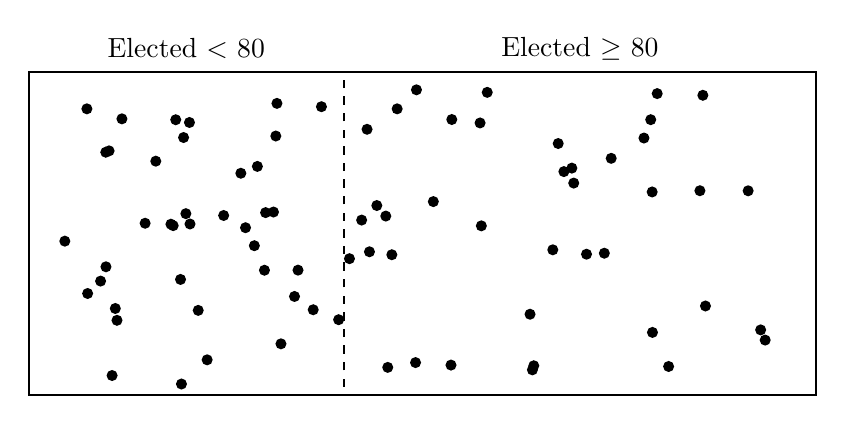
\begin{tikzpicture}
    % Draw the population rectangle
    \draw[thick] (-4,-0.1) rectangle (6,4);
    % Divide the rectangle into two parts
    \draw[thick, dashed] (0,0) -- (0,4);

    % Label the parts
    \node at (-2,4.3) {Elected $<$ 80};
    \node at (3,4.3) {Elected $\geq$ 80};

    \pgfmathsetseed{42} % set random seed
    % Draw random dots
    \foreach \i in {1,...,40} {
        \pgfmathsetmacro{\xone}{0-abs(3.5*rand)-0.05}
        \pgfmathsetmacro{\yone}{abs(3.8*rand)}
        \pgfmathsetmacro{\xtwo}{0+abs(5.9*rand)+0.05}
        \pgfmathsetmacro{\ytwo}{abs(3.8*rand)}
        \fill[black] (\xone, \yone) circle (2pt);
        \fill[black] (\xtwo, \ytwo) circle (2pt);
    }
\end{tikzpicture}
\end{center}
\pause
\end{frame}
%%-----
\begin{frame}
\frametitle{Classical Probability in the Context of Elections}

\begin{itemize}
    \item What is the probability that a candidate younger than 80 years old is elected?\pause
\end{itemize}

    $$P(Elected<80) = \frac{\text{\# (Favorable Cases)}}{\text{\# (Total Cases)}} = \frac{\text{Count of Red Dots}}{\text{Total Number of Dots}}$$\pause

\begin{center}
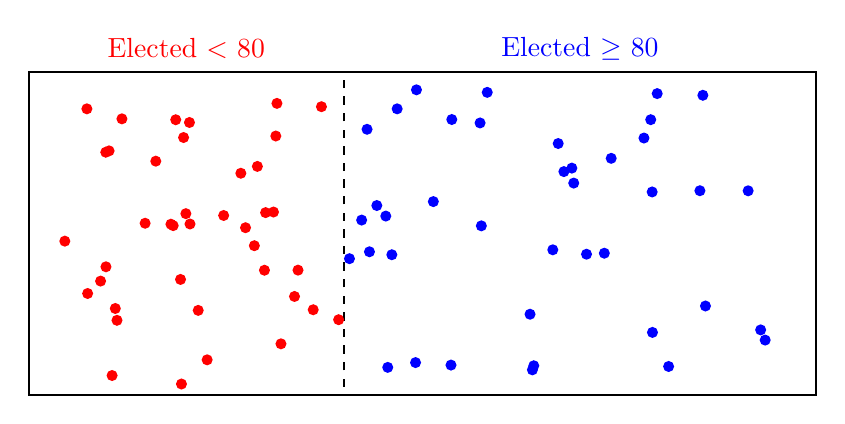
\begin{tikzpicture}
    % Draw the population rectangle
    \draw[thick] (-4,-0.1) rectangle (6,4);
    % Divide the rectangle into two parts
    \draw[thick, dashed] (0,0) -- (0,4);

    % Label the parts
    \node at (-2,4.3) { \textcolor{red}{Elected $<$ 80} };
    \node at (3,4.3) { \textcolor{blue}{Elected $\geq$ 80} };

    \pgfmathsetseed{42} % set random seed
    % Draw random dots
    \foreach \i in {1,...,40} {
        \pgfmathsetmacro{\xone}{0-abs(3.5*rand)-0.05}
        \pgfmathsetmacro{\yone}{abs(3.8*rand)}
        \pgfmathsetmacro{\xtwo}{0+abs(5.9*rand)+0.05}
        \pgfmathsetmacro{\ytwo}{abs(3.8*rand)}
        \fill[red] (\xone, \yone) circle (2pt);
        \fill[blue] (\xtwo, \ytwo) circle (2pt);
    }
\end{tikzpicture}
\end{center}

\end{frame}



% Slide 5
\begin{frame}{Three Axioms of Probability - Introduction}
\vspace{1cm}
    \begin{block}{Probability Function}
    Probability is a real-valued function \(P\) that assigns to each event \(A\) in a sample space \(S\) a number known as the \textbf{probability of the event \(A\)}, denoted by \(P(A)\).
    \end{block}\pause
\vspace{2cm}

\textcolor{gray}{\scriptsize An axiom in mathematics is a foundational statement assumed to be true, serving as a building block for the branch of mathematics in question. In probability and statistics, our theory is based upon three axioms.}


\end{frame}

% Slide 6
\begin{frame}{Three Axioms of Probability - Detailed}
    The function \(P\) satisfies the following properties (axioms):\pause
    \begin{enumerate}
        \item \(P(A) \geq 0\) for any event \(A\). (Nonnegativity)\pause
        \item \(P(S) = 1\), where \(S\) is the sample space. (Certainty)\pause
        \item For any sequence, \(A_1, A_2, \ldots A_k\), of mutually exclusive events, i.e., $A_j \cap A_i =\emptyset$, , \[P\left(A_1 \cup A_2 \cup A_3 \cdots \cup A_k \right) = P(A_1)+P(A_2)+P(A_3) + \cdots + P(A_k)\] (Additivity)\pause
    \end{enumerate}
    \vspace{2em}
    These axioms form the basis of probability theory, providing a foundation for all subsequent probability rules.
\end{frame}

% Slide 7.1
\begin{frame}{Probability Distributions for Finite Sample Spaces}
    Probability distributions describe how probabilities are assigned across all possible outcomes in a finite sample space. \\ \pause
\vspace{2em}
    \textbf{Definition:}
    A probability distribution assigns a probability \( P(a) \) to each outcome \( a \) in the sample space such that:\pause
    \begin{itemize}
        \item \( P(a) \geq 0 \) for each outcome \( a \)\pause
        \item The sum of probabilities for all outcomes is 1, \( \sum_{a \in S} P(a) = 1 \) \pause \nonumberfootnote{\tiny The symbol $\in$ is used to construct a statement in set theory notation, and it means ``belongs to'' or ``is an element of.'' Imagine the set $S=\{a,b,c,d\}$, therefore the statement ``$a \in S$'' is true because $a$ is an element of $S$.}
    \end{itemize}

\end{frame}

\begin{frame}{Probability Mapping: \(P: S \to [0,1]\)}
    \begin{center}
    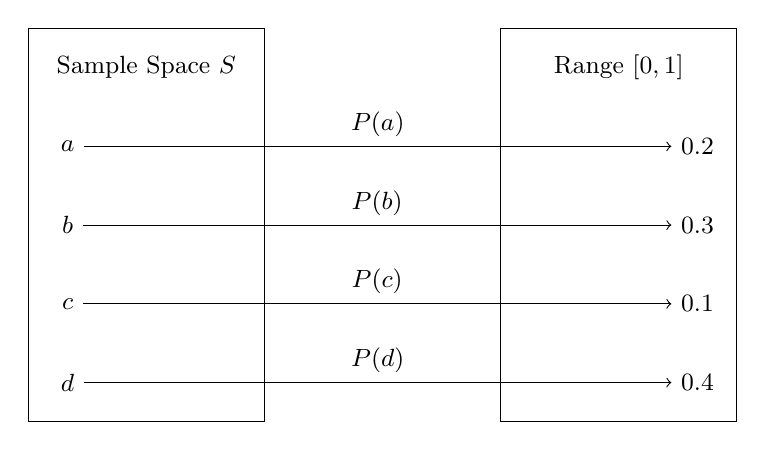
\begin{tikzpicture}[every node/.style={font=\small}]
        % Left rectangle: Sample Space S
        \node[draw, rectangle, minimum width=3cm, minimum height=5cm] (S) at (0,0) {};
        \node at (0,2) {Sample Space \(S\)};

        % Elements in S
        \node (a) at (-1,1) {\(a\)};
        \node (b) at (-1,0) {\(b\)};
        \node (c) at (-1,-1) {\(c\)};
        \node (d) at (-1,-2) {\(d\)};

        % Right rectangle: Range [0,1]
        \node[draw, rectangle, minimum width=3cm, minimum height=5cm] (R) at (6,0) {};
        \node at (6,2) {Range \([0,1]\)};

        % Probability values inside R
        \node (pa) at (7,1) {\(0.2\)};
        \node (pb) at (7,0) {\(0.3\)};
        \node (pc) at (7,-1) {\(0.1\)};
        \node (pd) at (7,-2) {\(0.4\)};

        % Arrows indicating the mapping P: S -> [0,1]
        \draw[->] (a) -- (pa) node[midway, above] {\(P(a)\)};
        \draw[->] (b) -- (pb) node[midway, above] {\(P(b)\)};
        \draw[->] (c) -- (pc) node[midway, above] {\(P(c)\)};
        \draw[->] (d) -- (pd) node[midway, above] {\(P(d)\)};
    \end{tikzpicture}
    \end{center}
\end{frame}


\begin{frame}
    \frametitle{Probability Problem: Number of Heads When Throwing Two Coins}

    \textbf{Problem Statement:}
    \begin{itemize}
        \item We toss \textbf{two fair coins}.
        \item We define an \textbf{event} as a specific \textbf{number of heads} observed.
        \item Our goal is to determine the probability distribution of the different realizations of this outcome.
    \end{itemize}

    \textbf{Sample Space:} The possible outcomes of flipping two fair coins are:
    \[
    S = \{ HH, HT, TH, TT \}
    \]
    where:
    \begin{itemize}
        \item \(HH\): Both coins land on heads.
        \item \(HT\) and \(TH\): One coin lands on heads, the other on tails.
        \item \(TT\): Both coins land on tails.
    \end{itemize}

\end{frame}

\begin{frame}
    \frametitle{Computing the Probability Distribution of \(X\)}

    \textbf{Step 1: Count the Outcomes for Each Event}
    \begin{itemize}
        \item \(X = 0\) (No heads): \( \{TT\} \) → 1 outcome \pause
        \item \(X = 1\) (One head): \( \{HT, TH\} \) → 2 outcomes \pause
        \item \(X = 2\) (Two heads): \( \{HH\} \) → 1 outcome
    \end{itemize}

    \textbf{Step 2: Compute Probabilities}
    \vspace{-2em}
    \begin{center}
        \begin{tabular}{c|c|c}
            \(X\) (Number of Heads) & Favorable Outcomes & Probability \( P(X) \) \\
            \hline
            0 & \( TT \) & \( 1/4 = 0.25 \) \\  \pause
            1 & \( HT, TH \) & \( 2/4  = 0.50 \) \\  \pause
            2 & \( HH \) & \( 1/4  = 0.25 \) \\  \pause
        \end{tabular}
    \end{center}

    \textbf{Final Answer:} The probability distribution of the event is:

    \makebox[\textwidth]{ % Expands the box to the full width
   $$
    P(\text{Zero Heads}) = 0.25, \quad P(\text{Just One}) = 0.50, \quad P(\text{Two Heads}) = 0.25
    $$
    }

\end{frame}

\begin{frame}{Probability Distribution of the Total Number of Heads When Throwing Two Coins}
\vspace{1em}
\centering
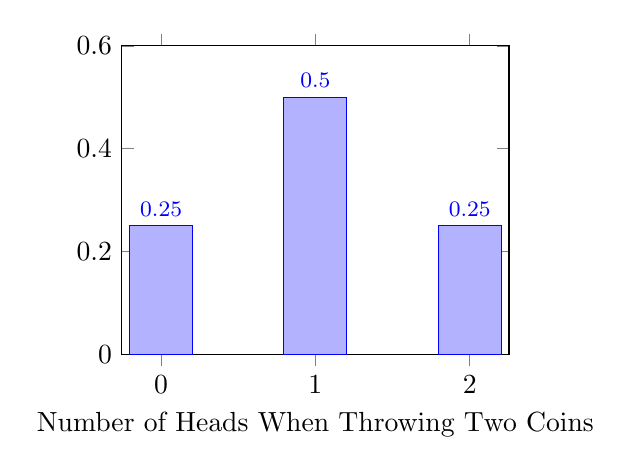
\begin{tikzpicture}
    \begin{axis}[
        ybar,
        bar width=0.8cm,
        symbolic x coords={0, 1, 2},
        xtick=data,
        ymin=0, ymax=0.6,
        xlabel={Number of Heads When Throwing Two Coins},
        yticklabel=\pgfmathprintnumber{\tick}, % Fix for scientific notation
        yticklabel style={
            /pgf/number format/fixed, % Forces normal decimal format
            /pgf/number format/precision=3 % Limits decimal places to 3
        },
        scaled ticks=false, % Prevents scientific notation
        nodes near coords,
        every node near coord/.append style={/pgf/number format/fixed,
            font=\footnotesize},
        width=6.5cm, height=5.5cm,
        enlarge x limits={abs=0.5cm},
    ]
    \addplot coordinates {(0,0.25) (1,0.50) (2,0.25)};
    \end{axis}
\end{tikzpicture}

\end{frame}



% Slide 7.2
\begin{frame}
\frametitle{Setting: Probability Distribution of Discrete Outcomes}
\begin{itemize}
    \item We analyze hypothetical (simulated) historical data of country pairs.\pause
    \item Each combination of variables (Democratic Regimes, Economic Interdependence, War) for a pair of two countries is an outcome.\pause
    \item We aim to calculate the probability distribution of these discrete outcomes.\pause
    \item Variables:\pause
    \begin{itemize}
        \item \textbf{Both Countries Are Democratic:} Yes/No (No = if at least one county of the pair is not a democracy)\pause
        \item \textbf{Economic Interdependence:} High/Low (Do the two countries share strong economic ties and transactions?)\pause
        \item \textbf{War:} Yes/No (Have the two countries ever been in a war against each other?)
    \end{itemize}
\end{itemize}
\end{frame}

% Slide 7.3 --- REPLACE THE EXAMPLE, USE SURVEY DATA INSTEAD
\begin{frame}{Summary of Dyadic (pairwise) Interactions}
    \begin{table}
    \centering
    \begin{tabular}{|
        >{\centering\arraybackslash}p{0.2\textwidth}|
        >{\centering\arraybackslash}p{0.2\textwidth}|
        >{\centering\arraybackslash}p{0.15\textwidth}|
        >{\centering\arraybackslash}p{0.15\textwidth}|
        >{\centering\arraybackslash}p{0.10\textwidth}|
    }
    \hline
    \textbf{Both Democratic} & \textbf{Economic Interdependence} & \textbf{War} & \textbf{Count} & \textbf{Prob.} \\
    \hline
    No & Low & Yes & 23 & 0.12 \\
    No & Low & No & 82 & 0.43 \\
    No & High & Yes & 4 & 0.02 \\
    No & High & No & 26 & 0.14 \\
    Yes & Low & Yes & 5 & 0.03 \\
    Yes & Low & No & 35 & 0.18 \\
    Yes & High & No & 15 & 0.08 \\
    Yes & High & Yes & 0 & 0.00 \\
    \hline
    \end{tabular}
    \caption{Probability distribution of randomly selecting one country pair combination. Total country pairs = 190.}
    \end{table}
\end{frame}

\begin{frame}{Venn Diagrams within the Universal Set}
\centering
\makebox[\textwidth]{
    \begin{columns}[t,onlytextwidth]
        % Left Column: Non-empty Intersection
        \column{0.5\textwidth}
        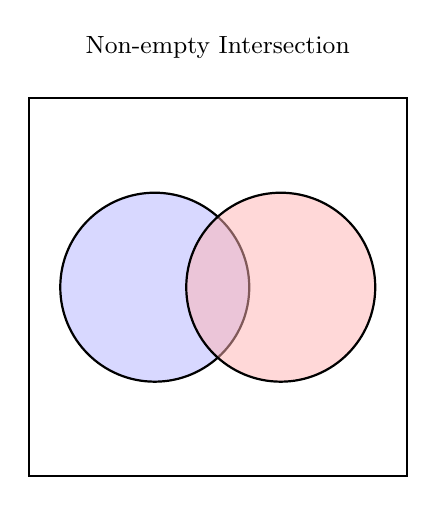
\begin{tikzpicture}[scale=0.8, every node/.style={font=\small}]
            % Universal set (square)
            \draw[thick] (-3,-3) rectangle (3,3);
            % Two circles with non-empty intersection
            \draw[thick, fill=blue!30, fill opacity=0.5] (-1,0) circle (1.5);
            \draw[thick, fill=red!30, fill opacity=0.5] (1,0) circle (1.5);
            % Diagram label
            \node at (0,3.8) {Non-empty Intersection};
        \end{tikzpicture}
        \pause
        % Right Column: No Intersection
        \column{0.5\textwidth}
        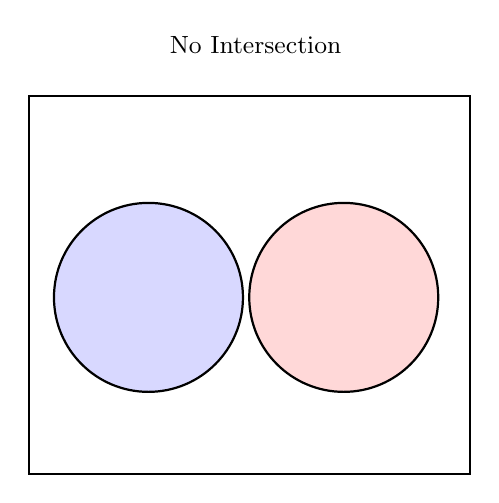
\begin{tikzpicture}[scale=0.8, every node/.style={font=\small}]
            % Universal set (square)
            \draw[thick] (-2.4,-2.8) rectangle (4.6,3.2);
            % Two circles with no intersection
            \draw[thick, fill=blue!30, fill opacity=0.5] (-0.5,0) circle (1.5);
            \draw[thick, fill=red!30, fill opacity=0.5] (2.6,0) circle (1.5);
            % Diagram label
            \node at (1.2,4) {No Intersection};
        \end{tikzpicture}
    \end{columns}
    }
\end{frame}

% Slide: Probability of the Intersection of Two Events
\begin{frame}{Probability of the Intersection of Two Events}
    \centering
    \definitionbox{Probability of the Intersection of Two Events $(Def.)$}{
    \begin{block}{}
        Following the classical definition, the probability that the event \(A\) happens AND the event \(B\) happens is given by:\pause
        \begin{align*}
            P(A \cap B) = \frac{\# (\text{Both \(A\) and \(B\) happen})}{\# (\text{Total Cases in \(S\)})}
        \end{align*}
    \end{block}
    }
\end{frame}

% Slide: Probability of the Union of Two Events
\begin{frame}{Probability of the Union of Two Events}

\centering
    \definitionbox[1\textwidth]{Probability of the Union of Two Events $(Def.)$}{
    \begin{block}{}
        Following the classical definition, the probability that the event \(A\) happens OR the event \(B\) happens is given by:\pause
        \footnotesize{
        \begin{align*}
            P(A \cup B) = \frac{\# (\text{\(A\) and not \(B\)}) + \# (\text{\(B\) and not \(A\)}) + \# (\text{Both \(A\) and \(B\)})}{\# (\text{Total Cases in \(S\)})}
        \end{align*}
        }
    \end{block}
    }

\end{frame}



%%%%%%%%%%%%%%%%%%%%%%%%%%%%%%%%%%%%%%%%%%%%%%%%%%%%%%%%%%%%%%%%%%%%%%%%%%%%%%%%%%%%%
\section{Probability Rules}
\transitionslide{Probability Rules}


% Slide 8
\begin{frame}{Addition Rule for Disjoint Events}
    The addition rule for disjoint (mutually exclusive) events states that if two events \( A \) and \( B \) cannot occur at the same time, then the probability of \( A \) or \( B \) occurring is the sum of their probabilities.\pause

    \[ P(A \cup B) = P(A) + P(B) \]\pause

    Example:\pause
    \begin{itemize}
        \item Let $A$ be ``At least one country is not a democracy AND They have low economic dependence AND The country pair has never been been at war".\pause
        \item Let $B$ "Both countries are democratic AND they have low economic dependence AND they have never been at war."\pause
        \item $P(A \cup B) = P(A) + P(B) = 0.43 + 0.18 = 0.61$
    \end{itemize}

\end{frame}



% Slide for General Addition Rule
\begin{frame}{General Addition Rule for Probabilities}
    The general addition rule is used to find the probability that either of two events occurs.\pause

    \begin{block}{Formula}
        If \(A\) and \(B\) are any two events, then the probability that \(A\) or \(B\) occurs is given by:\pause
        \[
        P(A \cup B) = P(A) + P(B) - P(A \cap B)
        \]\pause
    \end{block}

    \textbf{Explanation:}\pause
    \begin{itemize}
        \item \(P(A \cup B)\) is the probability of either \(A\) or \(B\) occurring.\pause
        \item \(P(A) + P(B)\) adds the probabilities of \(A\) and \(B\) occurring.\pause
        \item Subtracting \(P(A \cap B)\) corrects for the double counting of the intersection, where both \(A\) and \(B\) occur.
    \end{itemize}
\end{frame}


% Slide with Venn Diagram
\begin{frame}{Venn Diagrams: Example.}
    \begin{minipage}{0.55\textwidth}
        \footnotesize
        Hypothetical \textbf{Dataset:} Comparative sample of countries. \\
        \textbf{Variables:} 1) Regime type (Democratic vs. Not Democratic), 2) Level of Economic Inequality (High vs. Low).
        \vspace{0.5em}

        \begin{table}[hbtp]
        \centering
        \scriptsize
        \settowidth\tymin{\textbf{Inequality}}
        \setlength\extrarowheight{2pt}
            \begin{tabulary}{1.0\textwidth}{lCCC}

                \toprule
                & \multicolumn{2}{c}{\textbf{Inequality}} & \textbf{Row Totals} \\
                \cmidrule(lr){2-3}
                \textbf{Regime} & \textbf{High} & \textbf{Low} & \textbf{Total} \\
                \midrule
                \textbf{Democratic}   & 0.18 & 0.42 & 0.60 \\
                \textbf{Not Democ.}    & 0.24 & 0.16 & 0.40 \\
                \midrule
                \textbf{Column Totals} & 0.42 & 0.58 & 1.00 \\
                \bottomrule
            \end{tabulary}
            \captionsetup{font=tiny}
            \caption{\tiny Joint Probability Distribution}
            \textbf{Question}: What is the probability that a randomly selected country is either Democratic or has Low Inequality?
        \end{table}
    \end{minipage}
    \begin{minipage}{0.45\textwidth}
        % Placeholder for future content
    \end{minipage}
\end{frame}

\begin{frame}{Example}
    \textbf{Example:}\\[0.5ex]
    Let \(A\) be “a country is a democracy” and \(B\) be “a country has low inequality.” Consider a scenario where:
    \begin{itemize}
        \item \(P(A) = 0.60\) (Probability of being a democracy),\pause
        \item \(P(B) = 0.58\) (Probability of having low inequality),\pause
        \item \(P(A \cap B) = 0.42\) (Probability of being both Democratic and having low inequality).\pause
    \end{itemize}

    Using the general addition rule:
    \[
    P(A \cup B) = P(A) + P(B) - P(A \cap B) = 0.60 + 0.58 - 0.42 = 0.76
    \]

    Thus, if we select a random country from the sample, the probability that it is either Democratic or has Low Inequality is 76\%.
\end{frame}

% Slide for Probability of the Complement
\begin{frame}{Probability of the Complement}

    \begin{block}{Derivation}
        Consider an event \(A\) and its complement \(A^c\). Since \(A\) and \(A^c\) are mutually exclusive and exhaustive, the addition rule gives:\pause
        \[
        P(A \cup A^c) = P(A) + P(A^c) - P(A \cap A^c)
        \]\pause
        Because \(A\) and \(A^c\) are mutually exclusive, \(P(A \cap A^c) = 0\). \pause Also, \(A \cup A^c\) covers the entire sample space, so \(P(A \cup A^c) = P(S) = 1\). \pause Thus:
        \[
        1 = P(A) + P(A^c)
        \] \pause
    \end{block}
    \pause
    \textbf{Consequently:}
    \[
    P(A^c) = 1 - P(A)
    \]
\end{frame}

\begin{frame}{Example: Law School Applications}
    \emph{Suppose a student estimates a 15\% chance of being accepted by any given law school. Assuming acceptance decisions are independent, how many schools should they apply to have a probability of getting accepted to at least one school be higher than 80\%?}
    \pause
\vspace{1em}
\footnotesize

    Let \( A \) be the event of being accepted to one particular school, so:
    \[
    P(A) = 0.15, \quad P(A^c) = 0.85.
    \]
    \pause
    If the student applies to \( n \) schools (assuming independent decisions), the probability of being rejected by all schools is:
    \[
    P(\text{no acceptances}) = (0.85) \times (0.85) \cdots \times (0.85)  = (0.85)^n.
    \]
    \pause
    Therefore, the probability of at least one acceptance is:
    \[
    P(\text{at least one acceptance}) = 1 - (0.85)^n.
    \]
    \pause
    We want this probability to be at least 80\%. If try for different $n$ we see that 10 is the minimum number of applications such that $P(\text{at least one}) \geq 0.80$
\end{frame}



\begin{frame}{Probability of Acceptance to At Least One School}

\makebox[\textwidth]{
    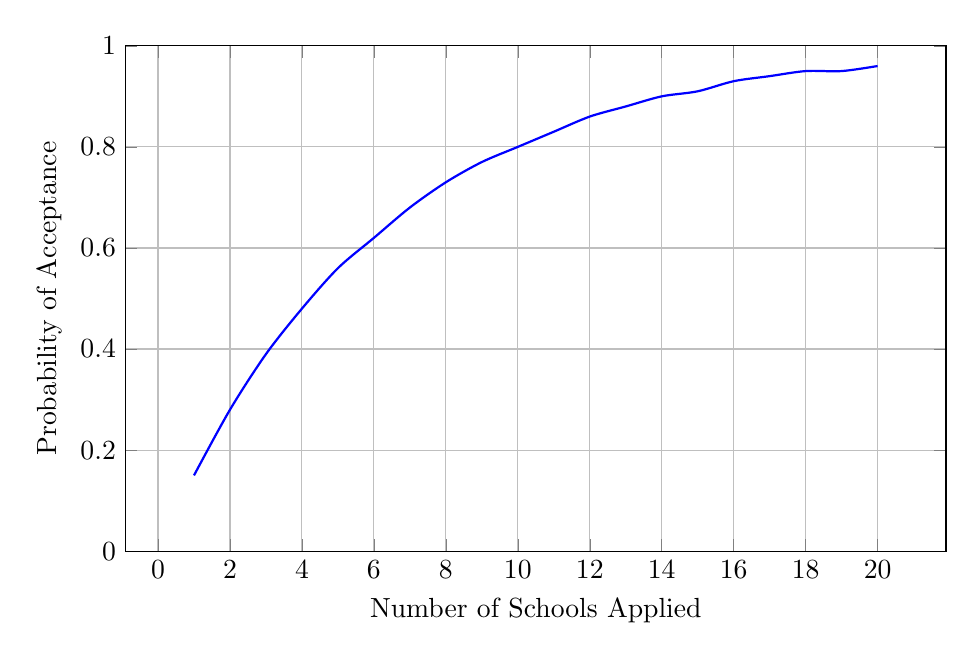
\begin{tikzpicture}
        \begin{axis}[
            xlabel={Number of Schools Applied},
            ylabel={Probability of Acceptance},
            ymin=0, ymax=1,
            grid=major,
            width=12cm,
            height=8cm
        ]
        \addplot[smooth,blue,thick] coordinates {
            (1,0.15)
            (2,0.28)
            (3,0.39)
            (4,0.48)
            (5,0.56)
            (6,0.62)
            (7,0.68)
            (8,0.73)
            (9,0.77)
            (10,0.8)
            (11,0.83)
            (12,0.86)
            (13,0.88)
            (14,0.9)
            (15,0.91)
            (16,0.93)
            (17,0.94)
            (18,0.95)
            (19,0.95)
            (20,0.96)
        };
        \end{axis}
    \end{tikzpicture}
}
\end{frame}

\begin{comment}

% Solve a problem
\begin{frame}{Example.}
    \begin{minipage}{0.4\textwidth}
        \scriptsize
        Hypothetical \textbf{Dataset:} All countries (each country is one observation). \\
        \textbf{Variables:} 1) Ranking of economic inequality (ordinal), 2) Whether the country is classified as a democracy (nominal).

    \begin{table}[hbtp]
        \centering
        \tiny
        \setlength\extrarowheight{2pt}
        \begin{tabulary}{1.0\textwidth}{LCCC}
            \toprule
            & \multicolumn{3}{c}{\textbf{Inequality}} \\
            \cmidrule(lr){2-4}
            & \textbf{Low} & \textbf{Medium} & \textbf{High} \\
            \midrule
            \textbf{Regime} & & & \\ \cmidrule(lr){1-1}
            \textbf{Full Democracy} & 0.12 & 0.08 & 0.04 \\
            \textbf{Flawed Democracy} & 0.04 & 0.12 & 0.08 \\
            \textbf{Electoral Autocracy} & 0.04 & 0.08 & 0.12 \\
            \textbf{Full Autocracy} & 0.04 & 0.04 & 0.17 \\
            \bottomrule
        \end{tabulary}
        \captionsetup{font=tiny}
        \caption{\tiny Joint Probability Distribution of Regimes and Economic Inequality}
    \end{table}

    \end{minipage}
    \begin{minipage}{0.2\textwidth}
        % Placeholder for future content
    \end{minipage}
    \begin{minipage}{0.3\textwidth}
        % Placeholder for future content
    \end{minipage}
\end{frame}

\end{comment}




\begin{frame}{Introduction to Conditional Probability}
    \textbf{Overview:}
    \begin{itemize}
        \item Conditional probability is a measure of the probability of an event occurring given that another event has already occurred.\pause
        \item This type of probability is essential in scenarios where the occurrence of one event affects the likelihood of another.\pause
    \end{itemize}

    \textbf{Concept:}
    \begin{itemize}
        \item Instead of considering all possible outcomes, conditional probability focuses only on the outcomes where a specific condition or event has occurred.\pause
        \item Useful in situations like medical testing, where we might be interested in the probability of a disease given a positive test result.
    \end{itemize}
\end{frame}

\begin{frame}{The Formula for Conditional Probability}
    \textbf{Conditional Probability Defined:}
    \begin{itemize}
        \item The probability of an event \( A \) given that event \( B \) has occurred is written as \( P(A|B) \).\pause
    \end{itemize}

    \textbf{Formula:}\pause
    \[
    P(A|B) = \frac{P(A \cap B)}{P(B)}
    \]\pause
    \begin{itemize}
        \item This formula assumes that \( P(B) > 0 \), i.e., the condition event \( B \) has a non-zero probability of occurring.\pause
        \item Note that $P(A|B) \neq P(B|A)$.
    \end{itemize}
\end{frame}

\begin{frame}{General Multiplication Rule}
\begin{itemize}
        \item Note that this gives a general formula for $P(A \cap B)$
        $$P(A \cap B) = P(A|B)\cdot P(B) = P(B|A)\cdot P(A)$$
    \end{itemize}
\end{frame}

\begin{frame}{Example: Using Conditional Probability}
    \textbf{Problem Setup:}
    \begin{itemize}
        \item We have a bag with 6 red and 4 blue marbles.
        \item We draw two marbles \textbf{without replacement}.
        \item We want the probability of drawing a blue marble first, then a red marble.
    \end{itemize}

    \textbf{Calculation:}
    \begin{itemize}
        \item Probability of drawing a blue marble first: \(\displaystyle \frac{4}{10}\).
        \item Probability of then drawing a red marble (given blue was drawn): \(\displaystyle \frac{6}{9}\).
        \item Combined probability:
        \[
         P(\text{Blue first, then Red})
         = \frac{4}{10} \;\times\; \frac{6}{9}
         = \frac{4}{15}.
        \]
    \end{itemize}
\end{frame}


% Slide 4: Example with a Probability Tree
\begin{frame}{Example: Probability Tree for Nuclear Weapon Investment}

We are studying two countries: Country 1 and Country 2. Each country decides whether to invest in nuclear weapons or not.\pause

\textbf{Probability Tree:}
    \begin{center}
    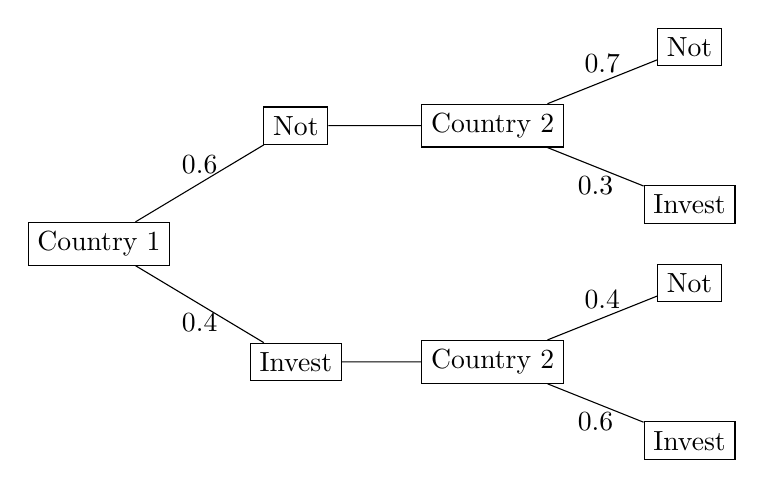
\begin{tikzpicture}[grow=right, level distance=2.5cm, sibling distance=3cm]
        \node[draw] {Country 1}
            child {
                node[draw] {Invest}
                [sibling distance=2cm]
                child {
                    node[draw] {Country 2}
                    child {
                        node[draw] {Invest }
                        edge from parent
                        node[below] {0.6}
                    }
                    child {
                        node[draw] {Not}
                        edge from parent
                        node[above] {0.4}
                    }
                }
                edge from parent
                node[below] {0.4}
            }
            child {
                node[draw] {Not}
                [sibling distance=2cm]
                child {
                    node[draw] {Country 2}
                    child {
                        node[draw] {Invest }
                        edge from parent
                        node[below] {0.3}
                    }
                    child {
                        node[draw] {Not }
                        edge from parent
                        node[above] {0.7}
                    }
                }
                edge from parent
                node[above] {0.6}
            };
    \end{tikzpicture}
    \end{center}

\end{frame}

\begin{frame}{Conditional Probability}

What's the probability of the event ``Country 2 invests in nuclear weapons ($\text{Invest}_2$), but Country 1 does not ($\text{Not}_1$)''

We can use the following rule: $P(A \cap B) = P(A) \cdot P(B|A) $
\vspace{0.5cm}

    \textbf{Calculation:}
    \begin{itemize}
        \item According to the respective branch of the tree: $P(\text{Invest}_2 | \text{Not}_1)=0.3$ \pause
        \item Also, \(P(\text{Not}_1) = 0.6\).\pause
        \item Thus, \(P(\text{Invest}_2 \cap \text{Not}_1) = 0.6 \times 0.3 = 0.18\).
    \end{itemize}

\end{frame}

% Slide 1: Independent Events - Definitions and Properties
\begin{frame}{Independent Events - Definitions and Properties}
    \textbf{Independent Events:}\pause
    \begin{itemize}
        \item Events \(A\) and \(B\) are independent if the occurrence of one does not affect the probability of the occurrence of the other.\pause
        \item Two events are independent if either:\pause
    \end{itemize}
    \[
    P(B|A) = P(B) \quad \text{(provided that } P(A) > 0\text{) or}
    \]\pause
    \[
    P(A|B) = P(A) \quad \text{(provided that } P(B) > 0\text{).}
    \]\pause
    \begin{itemize}
        \item Now, since independence tells us that \(P(B|A) = P(B)\), we can substitute \(P(B)\) in for \(P(B|A)\) in the formula given to us by the multiplication rule:\pause
    \end{itemize}
    \begin{center}
    $P(A \cap B) = P(A) \times P(B|A) = P(A) \times P(B)
    $ \pause
    \end{center}


\end{frame}

% Slide 2: Independent Events - Alternative Definition
\begin{frame}{Independent Events - \emph{Alternative} Definition}

    \begin{itemize}
         \item Given the previous result, events \(A\) and \(B\) are \textbf{independent events} if and only if:\pause
    \[
    P(A \cap B) = P(A) \times P(B)
    \]
    \vspace{-0.5cm}

    \pause
        \item Otherwise, \(A\) and \(B\) are called \textbf{dependent events}.\pause
        \item Recall that the ``if and only if" in the definition means that the if-then statement works in both directions, in ther words:\pause
        \begin{enumerate}
            \item If events \(A\) and \(B\) are independent, then \(P(A \cap B) = P(A) \times P(B)\).\pause
            \item If \(P(A \cap B) = P(A) \times P(B)\), then events \(A\) and \(B\) are independent.
        \end{enumerate}
    \end{itemize}
\end{frame}

% Slide: Definitions of P(A ∩ B) for Independent and Dependent Events
\begin{frame}{Definitions of \(P(A \cap B)\) for Independent and Dependent Events}

    \begin{minipage}[t]{0.45\textwidth}
        \centering
        \textbf{Independent Events}\pause
        \begin{block}{Definition}
            If events \(A\) and \(B\) are independent, then:\pause
            \[
            P(A \cap B) = P(A) \times P(B)
            \]\pause
        \end{block}
    \end{minipage}
    \hfill
    \begin{minipage}[t]{0.45\textwidth}
        \centering
        \textbf{Dependent Events}\pause
        \begin{block}{Definition}
            If events \(A\) and \(B\) are not independent, then:\pause
            \[
            P(A \cap B) = P(A) \times P(B|A)
            \]\pause
            or equivalently:
            \[
            P(A \cap B) = P(B) \times P(A|B)
            \]
        \end{block}
    \end{minipage}

\end{frame}


 % Slide 1: Law of Total Probability - Intuition
\begin{frame}{Law of Total Probability - Intuition}
    \textbf{Intuition:} \pause
    \begin{itemize}
        \item The Law of Total Probability helps us calculate the probability of an event by considering all possible ways that event can occur.\pause
        \item It involves breaking down the event into mutually exclusive cases by conditioning on a different event.\pause
        \item Consider the following example. What's the probability of randomly selecting one Senator and that they are woman?
    \end{itemize}
\end{frame}

\begin{frame}{Law of Total Probability - Example}

Define the events $B$ and $A$. We can split the event $B$ into two cases 1) $B$ and $A$ happen, and 2) $B$ and $A^c$ (not $A$) happens.  \newline
\vspace{0.5em}


Consider the following example. Assume $N_W$ current senators are woman. Define $O$ as the event ``a senator is older than 80 years.'' And define the event $W \cap O$ as the event ``A senator is woman \underline{and} older than 80 years.'' Hence, it must be the case that:
\begin{itemize}
    \item $N_W = N_{W\cap O} + N_{W\cap O^c}$
    \item Total Woman Senators = \# (Woman \& Older than 80) + \# (Woman \& Younger than 80).
    \item Assume that $N$ is the total number of senators. Then,
    \item $\frac{N_W}{N} = \frac{N_{W\cap O}}{N}+ \frac{N_{W\cap O^c}}{N}$
    \item $P(W) = P(W \cap O) + P(W \cap O^c)$.
\end{itemize}
\end{frame}

% set theory: B = (B \cap A) \cup (B \cap A^c). This is one rule.

% Slide 1: Law of Total Probability - Intuition
\begin{frame}{Law of Total Probability - Intuition}
    \textbf{Intuition:} \pause
    \begin{itemize}
        \item The Law of Total Probability calculates the probability of an event by breaking it down into the mutually exclusive cases the event can happen jointly with another.\pause
    \end{itemize}

    \textbf{Formula:}
    $$  P(B) = P(B \cap A) + P(B\cap A^c)  $$
    Alternatively, applying the general multiplication rule:
    $$ P(B) = P(B|A) \cdot P(A) + P(B|A^c) \cdot P(A^c) $$
    \pause

    \textbf{Explanation:}\pause
    \begin{itemize}
        \item \(P(B|A)\) is the probability of \(B\) given \(A\).\pause
        \item \(P(A)\) is the probability of \(A\).\pause
        \item \(P(A^c)\) is the complement of \(A\).
    \end{itemize}
\end{frame}

% Slide 2: Law of Total Probability - Example
\begin{frame}{Law of Total Probability - Example}
    \textbf{Example:}\pause
    \begin{itemize}
        \item Suppose we have two bags of marbles:\pause
        \begin{itemize}
            \item Bag One: 70\% red marbles, 30\% blue marbles.\pause
            \item Bag Two: 40\% red marbles, 60\% blue marbles.\pause
        \end{itemize}
        \item We randomly choose a bag, with a 50\% chance of picking either. What's the probability of drawing a blue marble ($B$)?
    \end{itemize}\pause

    \textbf{Calculation:}\pause
    \begin{itemize}
        \item Let \(A\) be the event of choosing Bag One, and \(A^c\) be the event of choosing Bag Two.\pause
        \item \(P(B|A) = 0.3\) (Probability of blue marble from Bag One)\pause
        \item \(P(B|A^c) = 0.6\) (Probability of blue marble from Bag Two)\pause
        \item \(P(A) = 0.5\), \(P(A^c) = 0.5\)         \pause
    \end{itemize}
    \begin{align*}
        P(B) &= P(B|A) \cdot P(A) + P(B|A^c) \cdot P(A^c) \\ \pause
        P(B) &= 0.3 \cdot 0.5 + 0.6 \cdot 0.5 = 0.15 + 0.3 = 0.45
    \end{align*}
\end{frame}

% example 2: use the previous tree and the law of t prob to calculate the prob that country 2 invests.


% Slide 1: Bayes' Theorem - Intuition and Example
\begin{frame}{Bayes' Theorem - Intuition and Example}
    \textbf{Intuition:}\pause
    \begin{itemize}
        \item Bayes' Theorem helps us update our beliefs (probabilities) based on new evidence.\pause
        \item \textbf{Prior:} The initial probability before seeing the new evidence.\pause
        \item \textbf{Posterior:} The updated probability after considering the new evidence.
    \end{itemize}
\end{frame}


% Slide 1: Bayes' Theorem - Intuition and Example
\begin{frame}{Bayes' Theorem - Intuition and Example}

    \textbf{Example:}\pause
    \begin{itemize}
        \item Suppose 2\% of politicians are corrupt (\(\Pr(C) = 0.02\)).\pause
        \item If a politician is corrupt, there is a 95\% chance they are mentioned in the Panama Papers (\(\Pr(PP|C) = 0.95\)).\pause
        \item If a politician is not corrupt, there is a 10\% chance they are mentioned in the Panama Papers (\(\Pr(PP|\neg C) = 0.1\)).\pause
    \end{itemize}

    \textbf{Problem:} Suppose it is found that a politician was mentioned in the Panama papers. What is the probability that they are corrupt? (i.e., compute \(\Pr(C|PP)\) ).
\end{frame}


% Slide: Bayes' Theorem - General Formula and Law of Total Probability
\begin{frame}{Bayes' Theorem - General Formula and Law of Total Probability}
    \textbf{Bayes' Theorem:}
    \[
    P(A|B) = \dfrac{P(B|A) \cdot P(A)}{P(B)} = \frac{P(B|A) \cdot P(A)}{P(B|A) \cdot P(A) + P(B|\neg A) \cdot P(\neg A)}
    \]\pause

    \textbf{Terms in Bayesian Nomenclature:}\pause
    \begin{itemize}
        \item \(P(A|B)\) is the posterior probability of \(A\) given \(B\).\pause
        \item \(P(B|A)\) is the likelihood of \(B\) given \(A\).\pause
        \item \(P(A)\) is the prior probability of \(A\).\pause
        \item \(P(B)\) is the marginal probability of \(B\), computed using the Law of Total Probability.\pause
    \end{itemize}
\end{frame}




% Slide 2: Bayes' Theorem - Formula and Calculation
\begin{frame}{Panama Papers and Corruption - Bayes Theorem}

    \textbf{Calculation:}
    \[
    Pr(P) = Pr(P|C) \cdot Pr(C) + Pr(P|\neg C) \cdot Pr(\neg C)
    \]\pause
    \[
    Pr(P) = (0.95 \times 0.02) + (0.1 \times 0.98) = 0.019 + 0.098 = 0.117
    \]\pause
    \[
    Pr(C|P) = \frac{P(PP|C) \times P(C)}{P(PP)} = \frac{0.95 \times 0.02}{0.117} \approx 0.162
    \]\pause
    \begin{itemize}
        \item The probability that a politician is corrupt, given a mention in the Panama Papers, is approximately 16.24\%.
    \end{itemize}
\end{frame}



\end{document}
